\section{Interest flooding mitigation methods}
\label{sec:design}

% Points what should be here:
% - What can be done (in general) to mitigate flooding attack
% - Which building blocks NDN architecture gives to mitigate Interest flooding attacks: Interest limits, ability to measure Interest satisfaction performance (Interest satisfaction stats)
% - Methods to set these limits: static/dynamic
% - Methods how limits can be applied: best-effort (fifo), "fair" queuing, probabilistic
% - Reference to caching: we don't consider it here, but caching provides additional level of protection, especially for certain types of attacks

% Our definition of attack mitigation is that good clients are still able to access data on the producer.

In this section we present several algorithms to mitigate Interest flooding attacks in NDN.  Our mitigation strategies feature varying degrees of implementation complexity and effectiveness---the higher the implementation complexity, the more effective is the algorithm against Interest flooding attacks. We start by describing our simple strategies and use the insights and lessons learned from the deployment of these to inform and design more effective mitigation techniques that works well in various topologies.

%   - Naive approach to Interest Limits (that is called physical limits everywhere else)
%     Example how this can be implemented in a simple way
%     Baseline solution
%   - Interest limits with "fair" queuing
%     Improving problem of simple limits (no single face can dominate), but doesn't solve the proble

% - Attack mitigation
%   - Per-incoming interface Interest statistics

%   - Dynamic Interests limit adjustments

%   - Probabilistic Interest accept

%The fact that each Data packet takes the reverse path of the corresponding Interest packet allows intermediate routers to match a received Data packet to the corresponding Interest packet and %thus determine which Interest packets were satisfied. As we describe in the rest of this section,  NDN routers can exploit this information to make informed decisions on which Interest packets to %forward, how many Interest packets to forward, and thus effectively defend against DDoS attacks.

%Our methods to mitigate Interest flooding attack rely on the fundamental principle of the NDN architecture: the flow balance between Interest and Data packets: one Interest packet (the only communication initiator) can be satisfied with at most one Data packet.
%Because NDN is host-to-host architecture (as opposed to end-to-end in the current IP Internet), the flow balance principle allow any entity on the network, end-hosts and routers, control what and how much Data they want to receive.
%Therefore, any node can limit the number of forwarded Interests, effectively limiting the amount of the retrieved Data.
%At the same time, each forwarded Interest can be used to build up various data plane performance statistics, such as per-incoming interface ratios of satisfied Interests.

%\subsection{Na\"{i}ve attack mitigation}

%We start with a couple of naive strategies that can be used to migitate attacks in an NDN network and describe the pitfalls associated with these strategies.

% In a normal network operation, the size of Interests packets is supposed to be significantly smaller than the size of the requested Data.

% All communication in NDN network is host-to-host and receiver-driven.

An obvious and na\"ive solution to defend against Interest flooding attacks is to restrict the number of Interests that are forwarded in the network. To this end, we exploit a 
 fundamental principle of NDN architecture---flow balance between Interest and Data packets. The flow balance refers to the fact that one Interest can be satisfied by at most one Data packet. This principle allows intermediate routers to control the inbound data traffic by controlling the number of outstanding Interests in the network. 
One simple implementation technique  is for an NDN router to limit the number of forwarded Interests out of each interface based on the physical capacity of the corresponding interface. This technique is a slight modification of the well-known {\it Token Bucket} algorithm that is currently widely used in packet-switched networks. Analogous to the {\it Token Bucket} algorithm, NDN routers keep track of the amount of data requested that can fully utilize the downstream link (estimated from the number of forwarded Interests) and once the link capacity limit has been reached, they no longer forward new incoming Interests. Ideally, the number of tokens (the pending \emph{Interests Limit}) for each link will be proportional to the link's bandwidth-delay product (BDP)~\cite{tcp-survey}. We can formalize this value as follows:
% With the objective to request as many Data packets, as downstream link can pump through, we are getting the following equation for Interest limit:
%
\begin{equation}
\small \mathrm{Interest\ Limit} = Delay\ [s] \cdot \frac{\mathrm{Bandwidth\ [Bytes/s]}}{\mathrm{Data\ packet\ size\ [Bytes]}}
\end{equation}

In the above equation, \emph{Delay} is the expected time of Interest being satisfied and \emph{Data packet size} is the size of the returned Data packet.
Although both these values are not known a priori, it is not really necessary to use their exact values.
One can simply set the pending Interest limit based on the average values of round trip time and observed Data packet size, as the network buffers can smooth out most of the network fluctuations.

This {\it Token Bucket} approach might be exceptionally restrictive in forwarding Interests---not all Interests will result in a Data packet---and might result in underutilization of the network. However, the biggest drawback of this algorithm is the fact that it can nourish DDoS attacks. If a router has utilized all its tokens to forward malicious Interests, it can no longer forward incoming Interests from legitimate users till the pending malicious Interests start to expire. One way to get around the issue is to impose a per interface limit, so that malicious Interests are not allowed to entirely consume the limits of a specific interface. We describe this technique in greater detail below.

%That is, if it is known that the amount of already requested data ($=$~amount of forwarded Interests) can fully utilize the downstream link, an NDN node---either an end-user or an NDN router---has absolutely no point in forwarding new incoming Interests and creating corresponding PIT entries.
%For example, if a router A on Fig.~\ref{fig:flooding example} already forwarded 125 Interests requesting 1000-byte Data packets, any new incoming Interests can be almost safely dropped, provided the link capacity between A--B is 100~Mbps and delay is 10~ms.
%In other words, 125 Data packets returned by router B will fully utilize the link ($125 \times 1000 \mathrm{~bytes} \approx 10\mathrm{~ms} \times 100\mathrm{~Mbps}$) and any excess Data would be dropped.
%
%\subsubsection{\textbf{Interest limits (physical limits)}}
%\label{sec:physical limits}
%
%\subsection{Physical limits}
\label{sec:physical limits}

The requirement to send an Interest in order to receive Data packet, provides an NDN consumer a unique opportunity to request the right amount of Data.
Moreover, the same opportunity to control the amount of data flow is given not only to consumers, but all routers between consumer and producer (or nearby caches).  
In other words, every node, either a consumer or an intermediate router, is able to control how much data it wants to receive by limiting the number of forwarded Interests.

The limitation can implemented in a number of different ways, including leaky bucket scheduling and window-based flow control.
We decided to following TCP-like window-based flow control and applied the sliding window approach to implement Interest limits.

The size of the window defines how many Interests can be send out before Interests get satisfied or expired.
From the one hand, this size should be large enough to ``fill the pipe,'' meaning that a node needs to send enough Interests to receive Data at full capacity of the incoming link.
On the other hand, the window's size should not be too large to avoid excessive buffering and congestion of the Data packet.
Thus, the ideal size for such a window need to be defined proportional to link's bandwidth-delay product~\cite{tcp-survey}.
With the objective to request as many Data packets, as downstream link can pump through, we are getting the following equation for Interest limit:

\[
\mathrm{Interest\ Limit} = Delay\ [s] \cdot \frac{\mathrm{Bandwidth\ [Bytes/s]}}{\mathrm{Data\ packet\ size\ [Bytes]}}
\]

Note that the value of \textit{Delay} is not known a priory and varies between different Interest-Data flows.
However, we do not need to know the exact value of the delay and can set it as an average round trip delay among all flows (with a reasonable filtering of outliers).
This way, the statistical traffic multiplexing with link-level buffering will allow full utilization of the downstream link.
Exactly the same reasoning can be applied to the \textit{Data packet size} parameter, which can also be set to an average observed Data packet size.

Unlike rate-based approaches, window-based limiting does not require precise knowledge about the rate, as well does not need precise scheduling mechanisms.
Like in TCP, the window-based flow is self-clocking, easily adjusting itself to any traffic patterns.

%%% Local Variables: 
%%% mode: latex
%%% TeX-master: "../paper"
%%% End: 


%%%%%%%%%%%%%%%%%%%%%%%
%%%%%%%%%%%%%%%%%%%%%%%
%%%%%%%%%%%%%%%%%%%%%%%

\subsubsection{\textbf{Token bucket with per interface fairness}}
\label{sec:queuing}

To address the lack of fairness associated with the na\"ive {\it Token Bucket} approach, we modify it to ensure that the Interests forwarded by a router on each interface represent a fair mix of Interests received from neighboring nodes. For example, in Fig.~\ref{fig:flooding example} router A can ensure that the tokens associated with Interests sent out on interface {\texttt eth2}  are fairly distributed across incoming interfaces \texttt{eth0} and \texttt{eth1}. 
%Due to the expected small volume of Interests, we cannot merely rely on network buffers to perform statistical multiplexing of Interests, as they would almost never be %buffered.
%At the same time, until bag of tokens is not empty, there is no reason to delay Interest forwarding, as we do not known how many and from which interfaces Interests %will arrive in the future.
In order to achieve our goal of ensuring ``fair'' mixing of Interests from all neighboring nodes, 
%, we implement an additional features to support buffering of Interests, if they cannot be immediately forwarded. 
we extend the Pending Interest Table to support flagging of Interests that cannot be immediately forwarded and implement hierarchical queues for each interface (see Fig.~\ref{fig:queueing}). 
This mechanism is essentially a class based queuing~\cite{floyd1995link}, with classes for each outgoing and incoming interface.
%As an alternative to hierarchical queues, one can also use an approach based on virtual time. For details, please see ~\cite{zhang1990virtual}.
We note that, unlike normal queuing, Interest queues do not actually store a packet, but merely a bi-directional pointer to the existing PIT entry.
Thus, a PIT entry can be quickly updated when the Interest is actually forwarded and the element can be easily removed from the queue when the Interest expires.

%For the buffering part, we can reuse Pending Interest Table, with a small extension to support flagging of the Interests that cannot be forwarded immediately (see example on Fig.~\ref{fig:queueing}). 
%As for the mixing part, we need an additional fair queuing mechanism, which can be implemented in a form of hierarchical queues (on Fig.~\ref{fig:queueing})\footnote{This essentially is a class based queuing, with classes for each outgoing/incoming interface.} or using virtual time approach~\cite{zhang1990virtual}. 

\begin{figure}[thb]
  \centering
  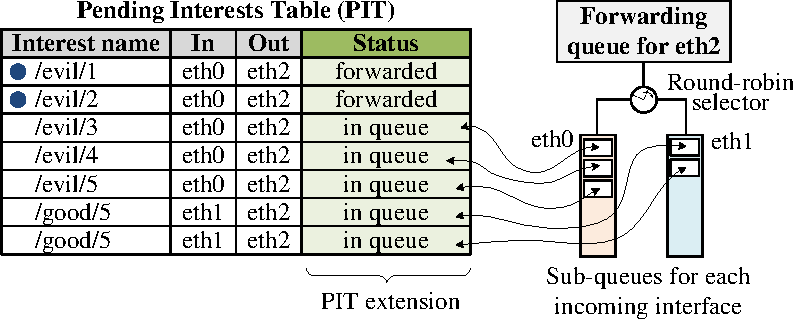
\includegraphics[scale=0.65]{queue}
  \vspace{-0.7cm}
  \caption{Interest queuing: if tokens are unavailable, the router creates a PIT entry, but instead of forwarding, it enqueues the Interest}
  \label{fig:queueing}
\end{figure}

We present a formalized description of this algorithm in Pseudocode~\ref{alg:queuing}. 
By setting appropriate queue sizes, we can control the amount of physical resources utilized at a router.
 % (such as memory and computation power). 
It is also important to set a sensible value for how long an Interest can be enqueued. 
If an Interest is enqueued for a long time, by the time it is dequeued and forwarded, the retrieved Data packet might be dropped at the downstream routers if their corresponding state expired. 
For our evaluations, we empirically chose to enqueue Interests up to 10\% of their original lifetime.
% We believe that implementing additional mechanisms on each pair of communicating routers to keep the Interests from getting stale would mitigate this issue, though the details are beyond the scope of this paper.
% Alex: I don't believe there is a need for separate discussion about "freshness", as we already introduced concept of lifetime
% {\color{red} \it Priya:  We need to  touch upon the Interest freshness issue in the NDN overview section; else we should get rid of this bit.}

%It should be noted that enqueued Interests should not be kept in the queue for a prolonged period of time.
%Otherwise, by the time the Interests reaches the Data, the state could have been long expired downstream, effectively making such an Interest useless.
%Additional mechanisms of pair-wise agreements between NDN routers and periodic Interest refresh can solve this particular problem, but it is out of the scope of the present paper.

%The algorithm extends the base Physical limits algorithm by enabling queuing when the bag of tokens is empty (lines 7--10), as well as by triggering an action (lines 16--21), when a token becomes available and enqueued Interest can be finally forwarded.
%At the same time, the algorithm limits number of Interests allowed in a queue, constraining memory usage increase by at most a constant factor, compared to the base Physical limits algorithm (i.e., memory attack on routers are still unfeasible). 


\floatname{algorithm}{\small Pseudocode}

%%%%%%%%%%%%%%%%%%%%%%%%%%%%%%
%%%%%%%%%%%%%%%%%%%%%%%%%%%%%%
%%%%%%%%%%%%%%%%%%%%%%%%%%%%%%

\begin{algorithm}[h]
\footnotesize
\caption{\small Token bucket with per interface fairness}
\label{alg:queuing}
\begin{algorithmic}[1]
\For{\textbf{each} interface \textbf{if}}
    \State{$L_{if} \leftarrow$ Interest Limit according to (1)}
    \State{$O_{if} \leftarrow 0$} \Comment{Outstanding Interests on interface \textbf{if}}
\EndFor

\vspace{0.1cm}

\Function{OutInterest}{Interest \textbf{i}, InInterface \textbf{in}, OutInterface \textbf{out}}
    \If{$L_{out} - O_{out} > 0$} \Comment{\textbf{out} is under limit cap}
        \State $O_{out} \leftarrow O_{out} + 1$  \Comment{``borrow'' a token from the bucket}
        \State add \textbf{out} to PIT entry and forward \textbf{i} to \textbf{out}
    \Else
        \State Queue $q \leftarrow out$.GetSubQueue($in$)
        \If{$Size(q) < L_{out}$}
           \State $q$.PushInterest($i$)
           \State add \textbf{out} to PIT entry, and link PIT entry with the queue
        \Else
           \State drop Interest
        \EndIf
    \EndIf
\EndFunction

\vspace{0.1cm}

\State{} \Comment{\textit{Whenever $L_{out} - O_{out}$ becomes larger than zero}}
\Function{TokenBecomesAvailable}{}
    \State Queue $q \leftarrow$ $out$.GetRoundRobinSubQueue 
    \State Interest $i \leftarrow$ $q$.PopInterest
    \State update PIT entry and Forward($i$, $out$)
\EndFunction

\vspace{0.1cm}

\Function{InData}{Data \textbf{d}}
   \State lookup PIT entry \textbf{p} for data \textbf{d}
   \For{\textbf{each} outgoing interface \textbf{out} in \textbf{p}}
        \State $O_{out} \leftarrow O_{out} - 1$ \Comment{``return'' token}
   \EndFor
\EndFunction

\vspace{0.1cm}

\Function{Timeout}{PIT entry $p$}
   \For{\textbf{each} outgoing interface \textbf{out} in \textbf{p}}
        \State $O_{out} \leftarrow O_{out} - 1$ \Comment{``return'' token}
   \EndFor
\EndFunction


\end{algorithmic}
\end{algorithm}


As we show in Section~\ref{sec:evaluation}, this algorithm provides partial relief from the Interest flooding attacks, allowing legitimate users to successfully fetch Data for 15--20\% of their expressed Interests. 
We note that while this algorithm might be reasonable for ensuring limited fairness in an NDN network, it is ineffective in protecting legitimate users from malicious ones. 
Attackers are able to successfully thwart access to content for legitimate users by sending a relatively modest volume of malicious Interests.


%At the same time, the Physical limits with or without fair queueing allows attackers to send a relatively small volume of Interests in order to significantly impact service for the legitimate users.
%Therefore, to successfully solve the problem, we need a fundamentally different, more intelligent approach, allowing localization of the attack traffic as close as possible to the attack origin.


%%%%%%%%%%%%%%%%%%%%%%%
%%%%%%%%%%%%%%%%%%%%%%%
%%%%%%%%%%%%%%%%%%%%%%%

The key drawback of the {\it Token bucket with per interface fairness} algorithm is that it still admits relatively large number of Interests from malicious users. A considerable percentage of these malicious Interests are forwarded all the way to content producers, thereby reducing resources available to serve legitimate users.  This algorithm attempts to ensure that each interface does not forward more than its fair share of Interests, but in doing so, it drops both legitimate and malicious Interests. For any strategy to be effective in defending against Interest flooding attacks, it must be able to detect and differentiate malicious requests from legitimate ones. 
% `Good' Interests from legitimate users must be admited and forwarded appropriately. 
Thus, the key question is how can we devise mitigation algorithms that allow a router to distinguish between `good' and `bad' Interests? 

%One can try a black- or whitelisting approach. However, besides the fact that source black- and whitelisting cannot work in %NDN as it does not feature source addresses, it requires extraneous knowledge to classify the incoming Interests.

%Priya: I have added the below point specifically to point out that a router cannot determine from the prefix name alone whether /parc is good  or bad...
  
%{\color{red} \textbf{Alex: This paragraph is confusing to me. I would remove it.} In NDN one cannot easily distinguish a `good' prefix from a `bad' one. Content producers must be able to support %dynamic generation of Data packets to satisfy incoming Interest packets---thus, an Interest that cannot be satisfied by matching Data from any intermediate router's cache is necessarily forwarded %to the producer for possible dynamic Data packet generation. 
%Thus intermediate routers cannot determine if the prefix is `good' or `bad' based on the prefix name alone---DDoS mitigation techniques that rely on whitelisting or blacklisting of certain %namespaces  will be inefficient and likely ineffective. }

% Alex: I'm not sure that this part is relevant... The point I see is that blacklisting and whitelisting is not 100% effective, but it can be used in both worlds

% In today's host-based Internet architecture where DDoS mitigation techniques rely on blacklisting of ``dark'' IP prefixes or whitelisting of good IP prefixes.
% Unlike IP, in NDN one cannot easily distinguish a `good' prefix from a `bad' one. 
% Content producers must be able to support dynamic generation of Data packets to satisfy incoming Interest packets---thus, an Interest that cannot be satisfied by matching Data from any intermediate router's cache is necessarily forwarded to the producer for possible dynamic Data packet generation. 
% Thus intermediate routers cannot determine if the prefix is `good' or `bad' based on the name alone---DDoS mitigation techniques that rely on whitelisting or blacklisting of certain namespaces  will be inefficient and likely ineffective. 


\subsection{Intelligent attack mitigation}
\label{sec:intelligent mitigating}

%While the Interest limit is the key building block to suppress mechanisms of the Interest flooding attack, legitimate Interests need to be somehow prioritized and malicious Interests need to be somehow penalized in order to completely suppress the attack.
%That is, instead of processing Interests always based on the first-in-first-serve rule, NDN routers need some basis to treat the incoming Interests differently.
%Thus, the primary task in bringing intelligence to the Interest flooding attack mitigation is to proactively distinguish between legitimate and malicious Interests.

In order to distinguish between legitimate and malicious Interests, we leverage another unique feature of  NDN architecture---guaranteed symmetric flow of Interest and Data packets. Since a Data packet takes the reverse path of the corresponding Interest packet, a router is guaranteed to see if an Interest it forwarded resulted in a matching Data packet or timed out. %The only exception being if Interest/Data packets were lost along the way due to congestion in the network.
Since malicious Interests are not likely to bring data back (as discussed in Section~\ref{sec:interest-flooding}), this information can be utilized by routers in differentiating attack and legitimate traffic.  %Therefore, intermediate routers can classify the ones that brings data back as legitimate, while the ones that timed out can be marked as malicious.\footnote{Recall that in order to maximize effect of the Interest flooding attack, an adversary expresses a large volume of junk Interests (see Section~\ref{sec:interest-flooding}).}  
%Implications of other types of attacks are discussed in Section~\ref{sec:discussion}.}

This timeout-based differentiation method is reactive in nature: one cannot determine in advance if an Interest will result in a timeout or Data being retrieved. However, routers can proactively maintain up-to-date statistics of Interest satisfaction ratios (number of forwarded versus number of satisfied Interests), and use this statistic to determine whether an incoming Interest should be forwarded or dropped. For example, maintaining independent Interest satisfaction ratio statistics for each incoming interface is sufficient to reasonably predict whether an Interest received from a neighbor connected to this interface will result in a Data packet or a timeout if forwarded. Statistics can also be kept at finer granularities such as per outgoing interface, per name prefix, etc. that can further improve the estimates. A router's goal should be to prioritize Interests that bring Data back while quickly penalizing those that occupy resources but don't generate a Data stream in return. In order to allow negative statistics to build up fast and positive statistics deteriorate quickly, we use the standard exponentially weighted moving average, performed once a second with $\alpha$ coefficient $e^{-1/30}$, approximately corresponding to a 30-second averaging window.

%Choosing the right balance between these contradictory requirements is a challenge and we explore this topic further  in the evaluation section.  %{\color{red} \it Priya: we should address the one that works best such as exponentially weighted moving average in eval section - it doesn't belong %here.} 

%The devil is always in the details.
%From the one hand, such statistics needs to start penalizing adversaries as soon as possible (i.e., negative stats should build up fast).
%On the other hand, the positive statistics should not deteriorate too fast (i.e., positive stats should be relatively long-term).
%Our preliminary experiments showed that the standard exponentially weighted moving average, performed once a second with $\alpha$ coefficient $e^{-1/30}$, approximately corresponding to a 30-second averaging window, provides a good balance between the two contradictory requirements.

% \subsubsection{\textbf{Data plane performance tracking}}
% \label{sec:stats}

% Note that there is a condition (line 6 in Pseudocode~\ref{alg:probabilistic model}) to check if there is a valid statistics point.
% This condition is extremely important, because it first provides a basis to distinguish between known facts (i.e., good or bad satisfaction ratio for the incoming interface) and unknown facts (e.g., the first time an Interests arrives on the interfaces).
% Second, it gives an opportunity to recover from a bad history (history of unsatisfied Interests) after malicious Interests are ceased to flow in.
% Essentially, this recovery relies on statistics module to perform time-based invalidation of historical data (timely, but not too quickly\footnote{Otherwise, attackers may send short bursts of malicious Interests, successfully avoiding differential Interest treatment}).


Pseudocode~\ref{algo:interest stats} formally defines how statistics can be generated for  each incoming interface. Note that in order to ensure decaying of relative statistics (e.g., ratio between the number of unsatisfied and forwarded Interest), only unsatisfied statistics needs to be exponentially smoothed (lines 23--26).  

\floatname{algorithm}{\small Pseudocode}

%%%%%%%%%%%%%%%%%%%%%%%%%%%%%%
%%%%%%%%%%%%%%%%%%%%%%%%%%%%%%
%%%%%%%%%%%%%%%%%%%%%%%%%%%%%%

\begin{algorithm}[h]
\footnotesize
\caption{\small Interest satisfaction statistics}
\label{algo:interest stats}
\begin{algorithmic}[1]

\For{\textbf{each} interface \textbf{if}}
    \State $F_{if} \leftarrow 0$ \Comment{forwarded Interests from interface \textbf{if}}
    \State $\hat F_{if} \leftarrow 0$ \Comment{averaged value of $F_{if}$}

    \State $U_{if} \leftarrow 0$ \Comment{unsatisfied Interests from interface \textbf{if}}
    \State $\hat U_{if} \leftarrow 0$ \Comment{averaged value of $U_{if}$}
\EndFor

\vspace{0.1cm}
\Function{OutInterest}{Interest \textbf{i}, InInterface \textbf{in}}
  \State $F_{in} \leftarrow F_{in} + 1$
  \State record \textbf{\emph{in}} in the list of incoming interfaces for \textbf{\emph{i}}
\EndFunction

\vspace{0.1cm}
\Function{InterestTimeout}{Interest \textbf{i}}
    \State lookup the list of incoming interfaces for \textbf{\emph{i}}

    \For{\textbf{each} interface \textbf{if} in the list}
        \State $U_{if} \leftarrow U_{if} + 1$
    \EndFor
\EndFunction

\vspace{0.1cm}

\State {} \Comment{\textit{Exponentially weighted moving average smoothing}}
\Function{EWMA}{} \Comment{Every second}
\State $\alpha \leftarrow e^{-1.0/30.0}$  %\Comment{$\approx$ 30~sec average}

\For{\textbf{each} interface \textbf{if}}
    \State $\hat U_{if} \leftarrow \alpha \cdot \hat U_{if} + (1 - \alpha) \cdot U_{if}$ 
    \State $U_{if} \leftarrow 0$ 

    \If{$F_{if} > 0$} \Comment{To ensure decaying of ratio $U_{if}/F_{if}$}
        \State $\hat F_{if} \leftarrow \alpha \cdot \hat F_{if} + (1 - \alpha) \cdot I_{if}$ 
        \State $F_{if} \leftarrow 0$ \Comment{Reset counters}
    \EndIf
\EndFor

\EndFunction

\end{algorithmic}
\end{algorithm}


Fig.~\ref{fig:ratio example} illustrates the resulting dynamics of the statistic during and after an Interest flooding attack. The attack duration is from 10 to 70~seconds. Prior to start of the attack, the percentage of unsatisfied Interests is zero.  
The statistics build up rapidly as soon as Interests start to time out, which happens approximately one second after the start of the attack.%\footnote{Again, we are assuming that Interests are admitted for a maximum period one second.}
For the duration of the attack (10--70~seconds), the percentage of unsatisfied Interests is close to 100\%: 
when the ratio is close to 100\%, routers drop all incoming Interests, resulting in decaying of the statistics until a new Interest is admitted, which eventually brings statistics back near 100\% point.
Finally, the ratio exponentially decays after the attack ceases.

\begin{figure}[htbp]
  \centering
  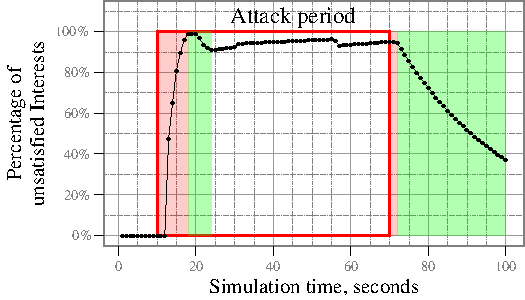
\includegraphics[scale=0.8]{limits}
  \vspace{-0.3cm}
  \caption{Dynamics of the unsatisfied Interests statistics on gateway's interface towards the attacker}
  \label{fig:ratio example}
\end{figure}

%%%%%%%%%%%%%%%%%%%%%%%
%%%%%%%%%%%%%%%%%%%%%%%
%%%%%%%%%%%%%%%%%%%%%%%

\subsubsection{\textbf{Satisfaction-based Interest acceptance}}
\label{sec:probabilistic}

Having successfully implemented a technique to gather statistics on Interest satisfaction ratios, our next challenge is in using this ratio to penalize malicious Interests. A straightforward method to achieve this enforcement is to use the Interest satisfaction ratio as the direct probability for accepting (forwarding) or rejecting an incoming Interest (see Pseudocode~\ref{alg:probabilistic model}).
%Apart from the Interest satisfaction statistics generation, there is a question how this statistics can be used to actually enforce prioritization and penalizing of Interests.


\floatname{algorithm}{\small Pseudocode}

%%%%%%%%%%%%%%%%%%%%%%%%%%%%%%
%%%%%%%%%%%%%%%%%%%%%%%%%%%%%%
%%%%%%%%%%%%%%%%%%%%%%%%%%%%%%

\begin{algorithm}[h]
\footnotesize
\caption{\small Satisfaction-based Interest acceptance}
\label{alg:probabilistic model}
\begin{algorithmic}[1]
\State{} \Comment{Same init, InData and Timeout functions as in Pseudocode~\ref{alg:queuing}}

\vspace{0.1cm}
\Function{OutInterest}{Interest \textbf{i}, InInterface \textbf{in}, OutInterface \textbf{out}}

    \State{} \Comment{Use uniform probability distribution model $P(X)$}
    \State{} \Comment{$P(X) : \forall x \in [0,1] \Rightarrow P(x) = x$}
    
    \If{$F_{in} > \theta $} \Comment{At least some Interests were forwarded before}
        \State $s \leftarrow (1 - U_{in} / F_{in})$
        \State Drop interest with probability $P(s)$
    \EndIf

    \State{forward the Interest, subjecting to token bucket limits}
\EndFunction

\end{algorithmic}
\end{algorithm}

Parameter $\theta$ on line 5 of the Pseudocode~\ref{alg:probabilistic model} ensures that the probabilistic model is not enforced when the volume of Interests arriving at a particular interface is small. This step is critical to provide an opportunity for legitimate users to regain their share of resources after temporary Data delivery failures.

A drawback of the satisfaction-based Interest acceptance method is that each router on the path makes an independent decision on whether to forward or drop an Interest. 
As a result of these independent decisions,  the probability of legitimate Interests being forwarded decreases rapidly as the number of hops between the content requester and producer grows; worsening the Interest satisfaction statistics and resulting in further drops.
In example on Fig.~\ref{fig:flooding example}, the router A observes 50\% satisfaction rate for \texttt{eth1} and 0\% rate for \texttt{eth0}. 
At the same time, router B observes a 30\% satisfaction rate for its \texttt{eth0} interface.
Next time a legitimate Interest arrives at router A, it has a 50\% chance of being forwarded further, and if forwarded, it has only a $50\% \times 30\% = 15\%$ probability of being forwarded further towards the data producer. With each increasing hop in the network, the probability of being forwarded to the next hop decreases significantly. 
One way to prevent this overreaction and unfair penalization is to ensure that the decision taken at each router on whether to forward or drop the Interest is not independent of the decision taken at preceding routers. An explicit notification such as a gossip protocol between neighboring NDN routers might alleviate the problem, but we leave the design and evaluation of it to future work.
%{\color{red}Alex: we should state that it is out of scope of the paper to evaluate this issue}

%%%%%%%%%%%%%%%%%%%%%%%
%%%%%%%%%%%%%%%%%%%%%%%
%%%%%%%%%%%%%%%%%%%%%%%

\subsubsection{\textbf{Satisfaction-based pushback}}
\label{sec:dynamic limits}

% Differential treatment of Interests received from different interfaces can be achieved in a more elegant way, without reverting to probabilistic methods.

The previous algorithm---the satisfaction-based Interest acceptance---divides the available forwarding tokens among all interfaces in proportion to their Interest satisfaction ratios.
% Given the drawbacks of this algorithm, the same effect can be achieved without relying on probabilistic models. 
An alternate algorithm for proportional token distribution without overreaction is to enable and enforce explicit Interest limit for each incoming interface, where the value of the limit depends directly on the interface's Interest satisfaction ratio.
Routers need to announce these limits to their downstream neighbors, ensuring that any Interest forwarded from the downstream router is allowed to get through, resulting in genuine Interest satisfaction statistics.

The formal definition of the satisfaction-based pushback algorithm is presented in Pseudocode~\ref{alg:dynamic limits}, while Fig.~\ref{fig:dynamic limits example} illustrates how the algorithm will work in our example in Fig.~\ref{fig:flooding example}.
Assuming an initial token bucket limit $L=10$ and the current satisfaction ratio for router A is 50\% for \texttt{eth1} and 0\% for \texttt{eth0}, and for router B the ratio is 30\% for \texttt{eth0}, each node will set and announce the following  incoming interface limit $L'$: 
\begin{enumerate}
\item router B will set and announce the incoming interface limit $L'=3$;
\item router A, after receiving announcement from B will readjust its incoming interface limits to $L'_{eth1} = 1.5$ and $L'_{eth0} = 0$; and
\item both legitimate users and adversaries may either obey or ignore the announced limit, which will be in any case enforced by router A.
\end{enumerate}


\begin{figure}[htbp]
  \centering
  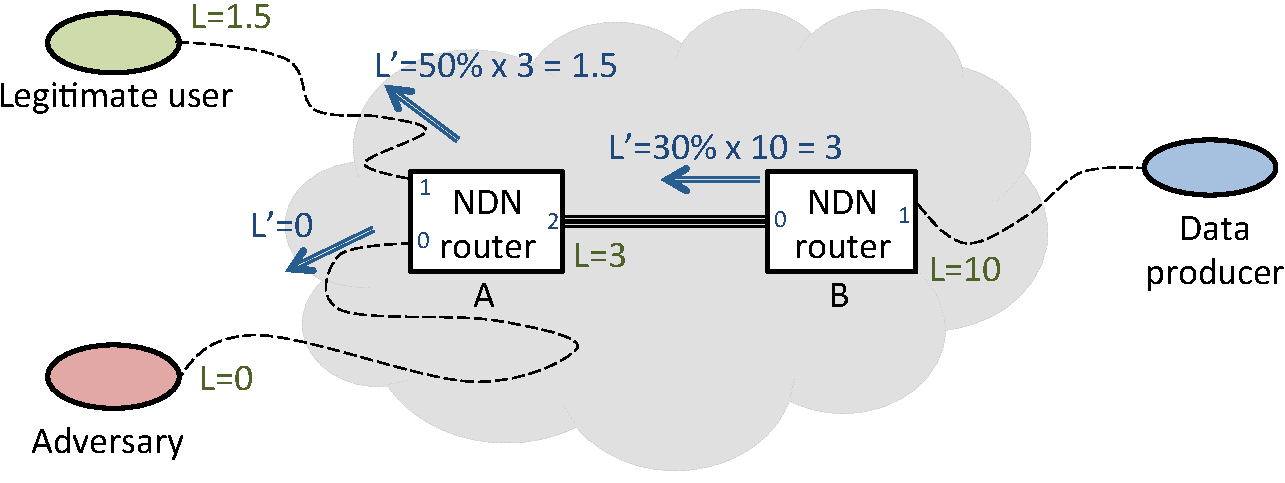
\includegraphics[scale=0.3]{dynamic-limits}
  \vspace{-0.3cm}
  \caption{Satisfaction-based pushback example
%: routers explicitly tell neighbors how many Interest packets they can deliver to the Data producer%
}
  \label{fig:dynamic limits example}
\end{figure}


\floatname{algorithm}{\small Pseudocode}

%%%%%%%%%%%%%%%%%%%%%%%%%%%%%%
%%%%%%%%%%%%%%%%%%%%%%%%%%%%%%
%%%%%%%%%%%%%%%%%%%%%%%%%%%%%%
{ 
\begin{algorithm}[h]
\footnotesize
\caption{\small Satisfaction-based pushback}
\label{alg:dynamic limits}
\begin{algorithmic}[1]
% \State{}\Comment{Same initialization, InData and Timeout functions as in Pseudocode~\ref{alg:queuing}}
\State{} \Comment{Same init, InData and Timeout functions as in Pseudocode~\ref{alg:queuing}}
\vspace{0.1cm}
\State{$\forall f \in \mathrm{interfaces} : L'_{f} \leftarrow L_{f}$} \Comment{Per-incoming interface Interest limit} 

\vspace{0.1cm}

\State{} \Comment{\textit{Announcement from the neighbor}}
\Function{InLimits}{InInterface $in$, Limit $L'$}
    \State $L_{in} \leftarrow L'$
\EndFunction

\vspace{0.1cm}

\Function{AnnounceLimits}{} \Comment{\textit{E.g., every second}}
\For{\textbf{each} outgoing interface $out$}

   \For{\textbf{each} incoming interface $in$}
        \State $L'_{in}= {L_{out}} \times (1 - U_{in}/F_{in})$
        \State AnnounceLimit($in$, $L'_{in}$)
   \EndFor

\EndFor
\EndFunction

\end{algorithmic}
\end{algorithm}


The zero limit for the adversary's link implies that  router A is temporarily not willing to accept any Interests from this interface until the statistics decay to the appropriate level (recall Fig.~\ref{fig:ratio example}).
At the next iteration of the satisfaction-based pushback algorithm, the legitimate user will be able to gradually improve the statistics on both routers A and B as all Interests from the user will get through and return Data, eventually resulting in a full allowance ($L'=L=10$) in the links between the routers A and B, and the user and router A.

We note that while in the description of the satisfaction-based pushback algorithm we explicitly used ``outgoing'' and ``incoming'' interfaces,  all interfaces can be both incoming and outgoing.
Thus, it may not be entirely clear which outgoing limit $L_{out}$ (line 10 in the algorithm) should be used to calculate the incoming limit $L_{in}$.
To overcome this problem, in our actual implementation we enforced separate incoming/outgoing interface limits for each individual FIB entry.
That is, for each FIB entry we set a separate Interest limit for each incoming interface (${L'}_{in}^{fib}$) based on a sum of FIB entry limits for each outgoing interface $L=\sum{L_{out}^{fib}}$.


Both satisfaction-based Interest acceptance and satisfaction-based pushback algorithms are forms of a well-known push-back mechanism~\cite{Pushback}, but with several core differences. 
First, we are suppressing (pushing back) unwanted requests for data, not actual data itself.
Second, differentiating between good and bad Interests is based on the traffic symmetry principle of NDN.
% Alex: I'm not entirely sure about this point... 
Finally, both intelligent attack mitigation algorithms can be deployed at all times without degrading network performance even when there are no active attackers. 

%%% Local Variables: 
%%% mode: latex
%%% TeX-master: "paper"
%%% End: 




